\documentclass[12pt]{article}
%compile using XeLaTeX
\usepackage{diary_style}
\setlength{\footskip}{\paperheight
  -(0.75in+\voffset+\topmargin+\headheight+\headsep+\textheight)
  -0.75in}

%\fontspec{Times New Roman}

\DeclareMathOperator{\di}{d\!}
\newcommand*\Eval[3]{\left.#1\right\rvert_{#2}^{#3}}

\begin{document}

%\doublespacing
\vspace{1.0 \baselineskip}

\begin{flushright}
	Alexander Caines\\
	MATH-310\\
	2-21-2020\\
\end{flushright}

\begin{center}
	\textbf{\underline{HMWK 4}}
\end{center}


%\vspace{0.5 \baselineskip}

\begin{enumerate}
	\item[*1]
		\begin{enumerate}
			\item[(*a)] Given that the bounds are  (-0.524, -0.288), which does not include 0, 
				it can be concluded that there is indeed a significant difference between the 
				indoor and outdoor concentrations of Hexavalent chromium.
				\begin{tcolorbox}[colback=white]
					\texttt{[1] indoor\_concentrations <- indoor[,2]}\\
					\texttt{[2] outdoor\_concentrations <- outdoor[,2]}\\
					\texttt{[3] sdi = sd(indoor\_concentrations)}\\
					\texttt{[4] sdo = sd(outdoor\_concentrations)}\\
					\texttt{[5] meandiff = mean(indoor\_concentrations - outdoor\_concentrations)}\\
					\texttt{[6] sddiff = sqrt(sdi\^2/length(indoor\_concentrations) + sdo\^2/length(outdoor\_concentrations))}\\
					\texttt{[7] zscore = qnorm(0.05)}\\
					\texttt{[8] b = meandiff - zscore*sddiff}\\
					\texttt{[9] a = meandiff + zscore*sddiff}
				\end{tcolorbox}
			\item[(b)] (-1.22, 0.404)
				\begin{tcolorbox}[colback=white]
					\texttt{[1] sdio = sd(indoor\_concentrations - outdoor\_concentrations)}\\
					\texttt{[2] z = qt(0.025, 32, lower.tail=FALSE)*sqrt(34/33)}\\
					\texttt{[3] lower\_bound = meandiff - sdio*z \# -1.22}\\
					\texttt{[4] upper\_bound = meandiff + sdio*z \# 0.404}\\
				\end{tcolorbox}
		\end{enumerate}
	\item[*2]
		\begin{enumerate}
			\item[(a)] The data appears to fall under a normal 
				distribution.
				\begin{figure}[!h]
					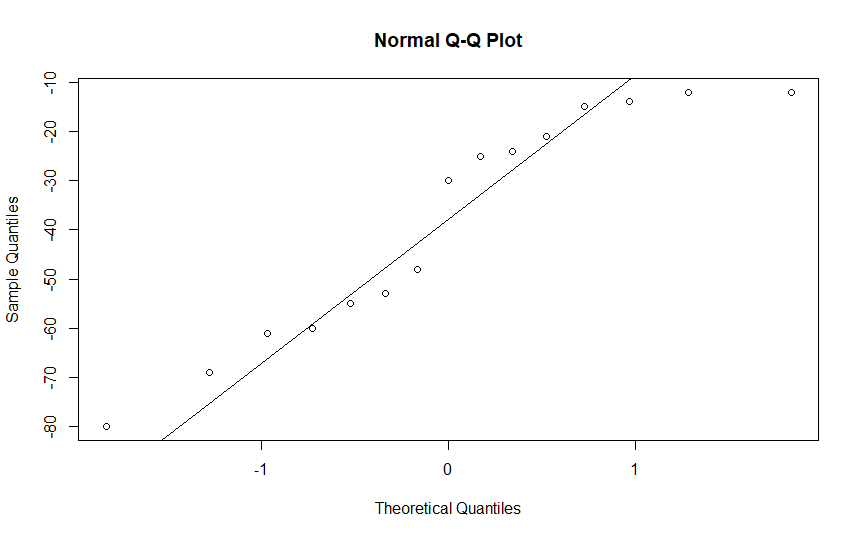
\includegraphics[width=\linewidth]{2b1.jpg}
				\end{figure}
				\newpage
			\item[(b)] The lower bound is -28.1
				\begin{tcolorbox}[colback=white]
					\texttt{[1] data <- c(-24, -12, -55, -15, -30, -60, -14, -21, -48, -12, -25, -53, -61, -69, -80)}\\
					\texttt{[2] means = mean(age)}\\
					\texttt{[3] z = qt(0.05, length(data)-1, lower.tail=TRUE)*(sd(data)/sqrt(length(data)))}\\
					\texttt{[4] means - z \# -29.05901}\\
				\end{tcolorbox}
			\item[(c)] The upper bound is 49.1
				\begin{tcolorbox}[colback=white]
					\texttt{[1] means + z \#49.14}
				\end{tcolorbox}
			\item[(d)] Pairing when the average difference = 0 does 
				not make any sense because then the age at onset 
				and the age at diagnosis would be the same.
			\item[(e)]  Given that  \texttt{t\_stat < table\_score}, the null hypothesis can be rejected.
				\begin{tcolorbox}[colback=white]
					\texttt{[1] t\_stat = (means + 25)/(sd(data)/sqrt(length(data))) \# -2.272445}\\
					\texttt{[2] table\_score = qt(0.05, length(data)-1, lower.tail=TRUE) \# -1.76131}\\
				\end{tcolorbox}
				
		\end{enumerate}
	\item[3]
		\begin{enumerate}
			\item[(a)] $H_0: p_2 = p_3, H_a: p_3 \neq p_2$
			\item[(b)] $p_3 - p_2$ or $\frac{x_3 - x_2}{n}$
			\item[(c)] $P := \frac{(x_2 - x_3)^2}{x_2 + x_3}$
			\item[(d)] Assuming a standard $\alpha$ level of 0.05, the true proportion of supporters are observed to have 
				increased given that the yield of the McNemar test was less than the alpha level (0.00815 < 0.05).
				\begin{tcolorbox}[colback=white]
					\texttt{[1] M <- matrix(c(350, 200, 150), nrow = 2)}
					\texttt{[2] mcnemar.test(M) \# Returns p-value of 0.00815}
				\end{tcolorbox}
			\item[(e)] Assuming a standard $\alpha$ level of 0.05, it cannot be concluded that the drug reduce migraine headaches as the 
				test statistic was greater than the McNemar test (-1.34 > -3.84).
				\begin{tcolorbox}[colback=white]
					\texttt{[1] x\_1 = 44, x\_2 =34, x\_3 = 46, x\_4 = 30}\\
					\texttt{[2] (x\_2 - x\_3)/sqrt(x\_2 + x\_3) \# -1.34}\\
					\texttt{[3] M <- matrix(c(x\_1, x\_2, x\_3, x\_4), nrow = 2)}\\
					\texttt{[4] mcnemar.test(m) \# -3.84}
				\end{tcolorbox}
		\end{enumerate}
	\item[4]
		\begin{enumerate}
			\item[(a)] Both the energizer and ultracell data has been 
				observed to be normal.
				\begin{figure}[!h]
					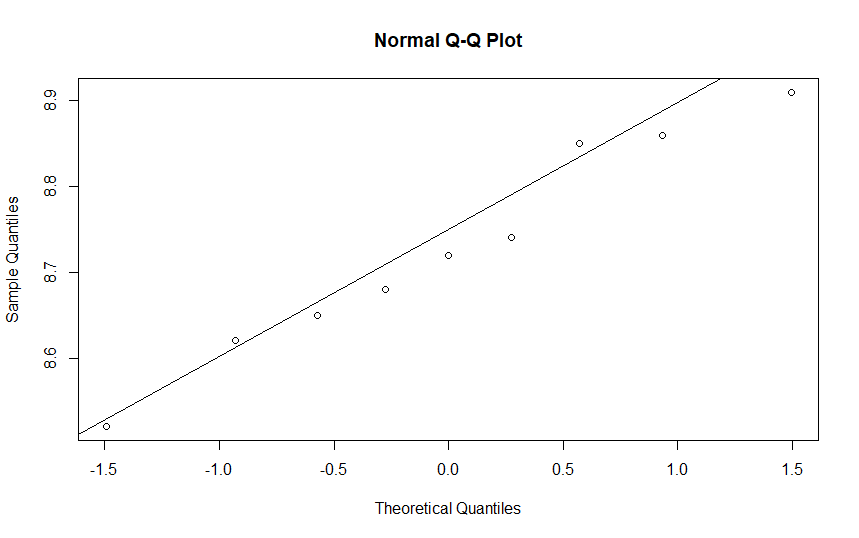
\includegraphics[width=\linewidth]{4a1.jpg}
				\end{figure}
				\begin{figure}[!h]
					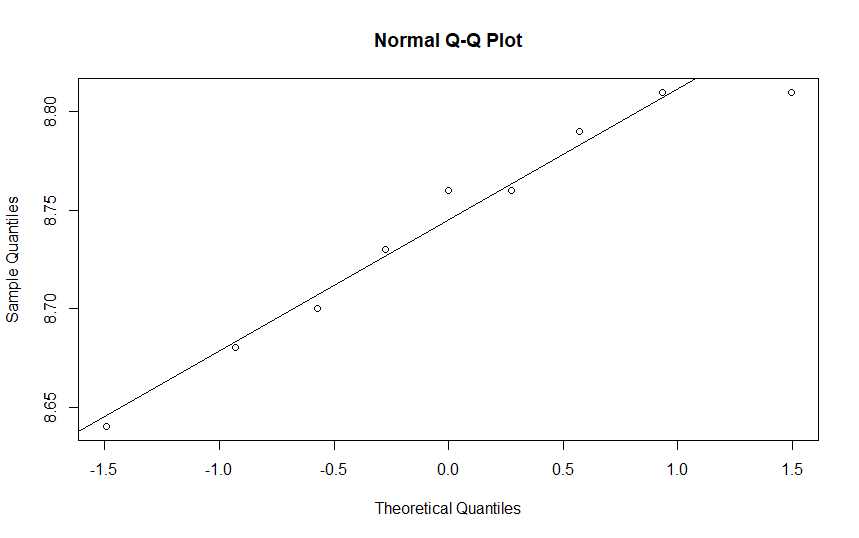
\includegraphics[width=\linewidth]{4a2.jpg}
				\end{figure}
			\item[(b)] Note that because the F statistic (4.55) is greater than the table score calculated (4.43), 
				it can be concluded that there is a significant difference between the variances of 
				the batteries.
				\begin{tcolorbox}[colback=white]
					\texttt{[1] ve = var(energizer)}\\
					\texttt{[2] vu = var(ultracell)}\\
					\texttt{[3] F = (ve/vu) \# 4.55}
					\texttt{[4] score = qf(0.025, 8, 8, lower.tail=FALSE) \# 4.43}
				\end{tcolorbox}
			\item[(c)] I would not pay the extra money because the 
				variance of the energizer batteries is too high.
		\end{enumerate}


\end{enumerate}

\end{document}
